\chapter{Diskussion}

In diesem Kapitel wird analytisch auf die vorangegangenen Resultate eingegangen und die Schwellenbestimmung der Rater und Software evaluiert. Im Zuge dessen werden die in Kapitel 1.3 aufgeführten Fragen chronologisch beantwortet:
%
\begin{tabbing}
	Ist die Spiroergometrie mit dem metabolicscan durchzuführen?\\
	Welche Methode zur Schwellenbestimmung ist optimal?\\
	Kann die VT2 mit den neuen Methoden genauer bestimmt werden, als mit RQ~=~1?
\end{tabbing}
%
Anschließend werden potentielle Fehlerquellen sowie eventuelle Defizite der Durchführung und Limitationen behandelt und diesbezüglich einige Vorschläge für die Firma cardioscan präsentiert.
%

\section{Spiroergometrie mit dem metabolicscan}

Da nach den Spiroergometrie-Tests für alle Probanden Plots generiert wurden, in denen die Veränderungen der \acs{VE}, \acs{VO2} und \acs{VCO2} erkennbar und nachvollziehbar waren, kann geschlussfolgert werden, dass der metabolicscan in Verbindung mit der \acs{CCPS} und Fahrradergometern grundsätzlich zur Durchführung eine Spiroergometrie genutzt werden kann. Während der Messungen wurden keine Störungen oder Fehler der verbauten Sensoren festgestellt. Die maximal gemessene Atemfrequenz bei den Testmessungen betrug \SI{52,5}{\per\minute} und liegt damit innerhalb der Grenzen des \acs{O2}-Sensors. Mit \SI{136,27}{\litre\per\minute} befindet sich auch die maximal gemessene \acs{VE} unterhalb des Maximums des Flowsensors. Der metabolicscan wurde vor dem Projekt mithilfe eines Lungensimulators bei Atemfrequenzen zwischen \SIlist{6;50}{\per\minute} und unterschiedlichen Gaskonzentrationen kalibriert, weswegen ausgeschlossen werden kann, dass die Sensoren fehlerhaft waren. Zudem wurde jeder bisher produzierte metabolicscan geprüft und mithilfe der Ergebnisse eine Ausgleichskurve für die Flowmessung entwickelt, die in die Gerätekalibrierung zu Beginn einer Messung implementiert ist. Dennoch können Abweichungen in der Messtechnik nicht vollkommen ausgeschlossen werden.\\
\clearpage
Alle Grafiken wurden bezüglich ihrer Qualität zunächst subjektiv und unbeeinflusst von anderen Personen in die Kategorien Gut und Kritisch einsortiert, um zu überprüfen, ob mit den Rohdaten des metabolicscan gute Plots zur Schwellenbestimmung erstellt werden. Plots, die optisch mithilfe einer jeweiligen Methode direkt auszuwerten waren und außerdem keine schwerwiegenden Artefakte aufwiesen, wurden als gut deklariert. In die Rubrik Kritisch kamen jene Graphen, die beispielsweise unregelmäßige Kurvenverläufe aufwiesen und dadurch nur sehr differenziert evaluiert werden konnten. Tab. \ref{tab:tabelle7} zeigt die Kategorien und Zuordnungen.
%
\begin{table}[H]
	\begin{center}
		\caption{Kategorisierung der Plots nach Qualität}
		\medskip
		\begin{tabulary}{\textwidth}{L L C C}
			\toprule
			& & Gut & Kritisch \\
			\midrule
			\midrule
			\multirow{3}{1.5cm}{\textbf{VT1}} & V-Slope & 7 & 21 \\
			& \acs{EQO2} & 13 & 15 \\
			\cmidrule{2-4}
			& \textsl{Summe} & 20 (36 \%) & 36 (64 \%) \\
			\midrule
			\multirow{3}{1.5cm}{\textbf{VT2}} & \acs{EQCO2} & 21 & 7 \\
			& \acs{VE}/\acs{VCO2} & 15 & 13 \\
			\cmidrule{2-4}
			& \textsl{Summe} & 36 (64 \%) & 20 (36 \%) \\
			\bottomrule
		\end{tabulary}
		\label{tab:tabelle7}
	\end{center}
\end{table}
%
Mit 64~\% wurde der Großteil aller Plots zur Bestimmung der VT1 als kritisch bewertet. 21 von 28 und damit 75~\% der V-Slope-Graphen war optisch schwierig auszuwerten. Mit 15 von 28 bzw. 54~\% wurde auch die absolute Mehrheit der \acs{EQO2}-Kurven so bewertet. Bei den Methoden zur VT2-Bestimmung fiel die Wertung andersherum aus und 75~\% der \acs{EQCO2}- und 54~\% der \acs{VE}/\acs{VCO2}-Plots wurden in die Kategorie Gut eingeordnet. Insgesamt waren 64~\% der VT2-Plots gut auszuwerten.
%
\subsection{Kriterien für die optische Bewertung der Plots}
%
Nachfolgend werden Eigenschaften aufgelistet, anhand derer ein einzelner Plot als gut deklariert wurde. Um gut auswerten zu können, mussten die V-Slope-Kurven und die dazugehörigen \acs{HF}-Kurven differenzierbar sein. Nur so konnte der überproportionale Anstieg der \acs{VCO2} erkannt werden. War diese Eigenschaft nicht erfüllt, wenn es beim V-Slope für einen X-Wert mehrere Y-Werte gab, so wurde der Graph als kritisch bezeichnet. Einige V-Slopes besaßen allerdings auch sehr dicht beieinander gelegene Messpunkte, sodass Steigungsänderungen optisch schwierig zu erkennen waren. Auch diese Plots wurden als kritisch kategorisiert.\\
Bei guten \acs{EQO2}-Kurven wurde für die VT1-Bestimmung erwartet, dass sie einen eindeutig zu detektierenden Tiefpunkt besaßen, auf den eine von dort an stetige Zunahme folgte. Wenn die Kurven jedoch Schwankungen innehatten oder aber mehrere, optisch auf relativ gleicher Höhe liegende Tiefpunkte aufwiesen, waren sie kritisch.\\
Ähnliches galt für die VT2-Bestimmung mittels \acs{EQCO2}. Gut waren die Graphen, die eine annähernd Badewannen-ähnliche Form besaßen, sodass im fortgeschrittenen Messverlauf ein deutlich sichtbarer Anstieg zu erkennen war. Es wurden bei den Tests jedoch auch Plots generiert, in denen diese Kurven ebenfalls Schwankungen aufwiesen, sodass mehrere, potentiell als VT2 assoziierbare \acs{EQCO2}-Steigungen existierten. Diese Grafiken galten als kritisch.\\
Für die \acs{VE}/\acs{VCO2} wurden ähnliche Voraussetzungen gestellt, wie für den V-Slope. Auch diese Graphen mussten differenzierbar sein und durften keine zackigen Verläufe annehmen. Auch hier sorgten einige Messpunkte mit optisch geringem Abstand für eine erschwerte, kritische Schwellenbestimmung. 
%
\section{Evaluierung der Methoden zur Schwellenbestimmung}
%
Die Kategorisierung wurde aus zeitlichen Gründen mit der ersten Version der grafischen Auswertung der Rohdaten vorgenommen. In Folge der Analyse der erstellten Grafiken wurde ein Fehler im MATLAB-Skript bei der Berechnung der \acs{AF} anhand des gemessenen Flows festgestellt. Dadurch könnte der V-Slope zur Bestimmung der VT1 verbessert werden. Hierzu müssten neue Testmessungen bzw. eine erneute Auswertung der neu generierten Plots durchgeführt werden, was jedoch der zeitliche Rahmen dieser Arbeit nicht zuließ. Dies zeigt jedoch bereits, dass eine weiterführende Optimierung der Algorithmen zu anderen Erkenntnissen führen kann.
%
\subsection{\acs{EQCO2} als optimale Methode}
%
75~\% der mit der ersten Algorithmus-Version generierten \acs{EQCO2}-Grafiken wurden jedoch bereits als gut kategorisiert. Die Ergebnisse dieser Methode brachte im Vergleich zwischen den Ratern sowie diesen und der Software die geringste mittlere Differenz der VT2 mit \SI{-3,02}{\per\minute} $\pm$\SI{6}{\per\minute} hervor (siehe. Abb. \ref{pic:pic26}). Als zusätzliches Vergleichsinstrument wurde aus den Ergebnissen von Ratern und Software der Korrelationskoeffizient $r$ für jede Methode bestimmt. Je dichter $r$ am Wert eins liegt, desto mehr korrelieren die Schwellenbestimmungen und desto eindeutiger ist die Methode zur Schwellenbestimmung anwendbar. Mit $0,912$ ist der Korrelationskoeffizient für das \acs{EQCO2} sehr nah am Wert 1 und im Vergleich mit den anderen Methoden am besten.
%
\begin{figure}[H]
	\centering
	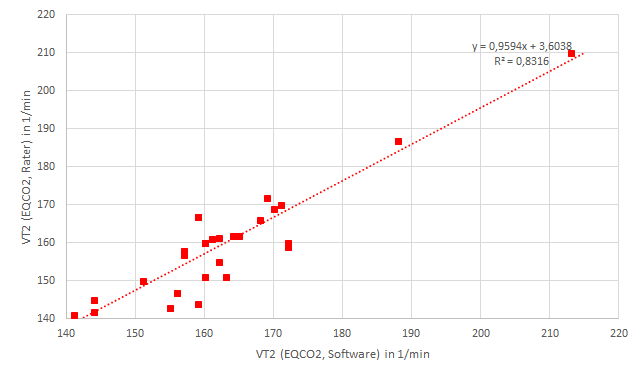
\includegraphics[scale=0.7]{Bilder/r_eqco2}
	\caption[Korrelation der \acs{EQCO2}-Werte von Ratern und Software]{Korrelation der VT2 mit \acs{EQCO2} von Ratern und Software in Form einer Regressionsgeraden; aufgetragen wird die gemittelte VT2 der Rater gegenüber der VT2 der Software in \si{\per\minute}}
	\label{pic:pic28}
\end{figure}
%
Die Regressionsgerade in Abb. \ref{pic:pic28} zeigt die gute Korrelation mit dem Bestimmheitsmaß $R^2 = 0,83$ zwischen Ratern und Software bei der mit \acs{EQCO2} bestimmten VT2 noch einmal grafisch.\\
Einen guten Plot zeigt beispielhaft Abb. \ref{pic:pic20}, bei der ein deutlicher Anstieg der \acs{EQCO2}-Kurve beobachtet werden kann. In Abb. \ref{subpic:pic3} ist zu sehen, dass die Differenzen zwischen den beiden Ratern und auch zwischen den Ratern und der Software im Allgemeinen dennoch relativ gering waren. Die drei Netze liegen, im Ganzen betrachtet, relativ häufig sehr nah übereinander. Abb. \ref{pic:pic26} zeigt dazu, dass bei lediglich fünf Probanden Differenzen >\SI{10}{\per\minute} zu beobachten sind.\\
Interessant ist allerdings, dass in Abb. \ref{pic:pic17} bei Probandin 6w ein solch eindeutiger Anstieg des \acs{EQCO2} zu sehen ist, Abb. \ref{subpic:pic3} jedoch entnehmbar ist, dass zwischen Rater 1 und Rater 2 sowie der Software eine relativ große Differenz bei der Schwellenbestimmung existiert. Rater 1 detektierte die VT2 eine Stufe früher, wo in Abb. \ref{pic:pic17} bereits ein \acs{EQCO2}-Anstieg in der orangen Kurve zu sehen ist. Dieser war für Rater 2 eventuell noch nicht signifikant. Die Software bestimmte die VT2 später, da der Wert mit den Referenzdaten der HUNT 3 Studie mehr übereinstimmte. Die Mittelung der Werte je Stufe könnte hier zu einem leichten Anstieg zwischen zwei Messpunkten führen, der noch nicht auf das Exzess-\acs{CO2} zurückzuführen ist. Die Oxygen Delay Time $\tau$ zwischen Steigerung der Leistung zu Beginn einer neuen Stufe und der respiratorischen Reaktion beträgt bei kleinen Inkrementen ca. \SI{45}{\second}~\cite{Kroidl.2015}. Bei einer Stufendauer von \SI{2}{\minute} kann somit davon ausgegangen werden, dass die physiologische Reaktion auf die Leistungssteigerung zu Beginn der Respirationsmessung nach \SI{90}{\second} bereits eingetreten ist. Vergleicht man die VT2 von Rater 1 bei \SI{130}{\per\minute} mit der \acs{HFmax} der Probandin bei \SI{178}{\per\minute}, entspricht die Schwelle 73~\%~\acs{HFmax}. Laut der HUNT 3 Studie liegt die durchschnittliche VT2 für gesunde Frauen zwischen 40 und 49 Jahren bei 90~\%~\acs{HFmax}$\pm$6~\%. Dementsprechend ist die VT2 von Rater 1 zu früh bestimmt worden.\\
Es gab wenige kritische \acs{EQCO2}-Kurven, in denen wechselnde Schwankungen zwischen positiver und negativer Steigung auftraten, sodass bei der optischen Auswertung die entscheidende \acs{EQCO2}-Zunahme nicht einfach erkennbar war. Dies ist beispielsweise bei Proband 8m in Abb. \ref{pic:pic18} der Fall. Die Kurve steigt im letzten Drittel des Plots zweimal an und fällt dazwischen einmal. Infolgedessen kam es zu unterschiedlichen Bestimmungen der VT2 durch die Rater, wie Abb. \ref{subpic:pic3} zeigt.
%
\subsection{\acs{VE}/\acs{VCO2} als geeignete Referenzmethode}
%
Die Abweichungen zwischen Ratern und Software beträgt für diese Methode im Mittel \SI{-4,07}{\per\minute} und die \acs{SD} $\pm$\SI{11}{\per\minute}. Verglichen mit der \acs{EQCO2}-Methode weisen die Ergebnisse größere Unterschiede auf und die Schwellenbestimmungen geschahen weniger eindeutig. Der Korrelationskoeffizient $r$ nimmt den Wert $0,816$ an. 15 von 28 Kurven für diese Methode waren gut. Ein Beispiel bietet Abb. \ref{pic:pic20} von Proband 20m. In der ersten Hälfte der Messung sind zwar einige sehr dicht gelegene Messpunkte zu erkennen, doch in der zweiten Hälfte, in der VT2 nur angenommen werden, ist die Zunahme der \acs{VCO2} deutlich zu sehen. Rater und Software kamen bei dieser Grafik zu sehr ähnlichen Ergebnissen.\\
Einige Kurven waren jedoch kritisch, da nicht differenzierbar. Bei dieser Methode wirkten diese Artefakte sich allerdings nicht so stark auf die Schwellenbestimmung aus, da sie, wie z.B. in Abb. \ref{pic:pic21} zu erkennen, ausschließlich in der ersten Messhälfte auftraten. Im Bereich der VT2 waren die Verläufe der Graphen meistens gut auszuwerten.\\
Jedoch traten auch in Feld 4 häufiger Plots auf, bei denen die Messpunkte dicht beieinander lagen und nicht genau ersichtlich war, in welcher Stufe der erste Anstieg auftrat. Hier kann beispielhaft Abb. \ref{pic:pic19} von Proband 9m gesichtet werden. Da der Graph in Feld 4 recht linear verläuft, war die subjektive Auswertung erschwert und die Rater bestimmten die VT2 später als die Software, die erneut den Vorteil der mathematischen Detektion der Steigung innehat.\\
Für die Auswertung von \acs{VE}/\acs{VCO2} lässt sich schlussfolgern, dass sie in Verbindung mit Mittelwerten und Stufentests erschwert wird, da der Graph anfällig für Artefakte ist. Eine \acs{SD} von $\pm$11 \si{\per\minute} zeigt, dass häufig keine eindeutigen Ergebnisse erzielt werden. Die Software birgt auch bei dieser Methode allerdings den Vorteil, dass die mathematische Bestimmung von Steigungsänderungen gut gelingt und die Methode somit für Vergleiche nutzbar wird. Eine erneute Auswertung mit einem optimierten Algorithmus könnte zu verbesserten und mehr korrelierenden Ergebnissen führen. Gegebenenfalls kann diese Methode künftig als Referenzmethode für die VT2-Bestimmung in die Software integriert werden.
%
\subsection{Problematik bei der Bestimmung der VT1}
%
\subsubsection{V-Slope-Methode}
%
Wenn die V-Slopes und die zugeordneten \acs{HF}-Kurven nicht differenzierbar waren, wie beispielsweise ist den Plots in Abb. \ref{pic:pic18} und Abb. \ref{pic:pic21} erkennbar ist, war die subjektive Bestimmung der VT1 erschwert und die Grafik kritisch. Diese Problematik trat relativ häufig auf und wurde auch vom 2.~Rater moniert. Es lagen jedoch auch Grafiken vor, bei denen die Plots zwar differenzierbar waren, aber dennoch mehrere Schwankungen aufwiesen.\\
Ein Beispiel hierfür ist die Grafik von Proband 8m. In Abb. \ref{pic:pic18} ist ein nicht differenzierbarer V-Slope zu sehen, der mehrere Knickpunkte enthält. Eine Vielzahl an solchen Punkten begünstigt eine große Varianz an Werten für die VT1. Während Rater~1 den ersten Anstieg in der 2. Stufe bei \SI{120}{\per\minute} beobachtete, wurde er laut Rater~2 erst nach den Schwankungen der Werte in Stufe 6 bei \SI{155}{\per\minute} erkennbar. Die kritische Bewertung des Plots wird dadurch belegt. Abb. \ref{subpic:pic1} zeigt hierzu, dass Rater~1 und Rater~2 häufiger, wie bei Proband 8m, zu unterschiedlichen Ergebnissen kamen.\\
Auch differenzierbare und stetig steigende V-Slopes, die jedoch viele Messpunkte besaßen und dadurch stärker geglättet wurden, brachten ungleiche Ergebnisse durch Rater und Software hervor. Für Proband 9m bestimmte Rater~1 die VT1 früher als Rater~2 und die Software. Bei Betrachtung von Abb. \ref{pic:pic19} fällt auf, dass die Kurvenverläufe allgemein recht eben sind. Hier wird ein Vorteil der algorithmischen Auswertung deutlich, da die Software die größte Steigungsänderung mathematisch und daher eindeutig bestimmt. Allerdings erkennt sie Software keine eventuellen Ausreißer und kann den Trainingszustand einer Person nicht bewerten, der die Rater dazu veranlassen konnte, die VT1 im späteren Messverlauf zu vermuten.\\
21 von 28 V-Slope-Grafiken waren aufgrund dieser Gründe kritisch, was durch das Diagramm in Abb. \ref{subpic:pic1} und die darin sichtbaren Abweichungen zwischen den Schwellen belegt werden kann. Es ist durch recht viele hellrote Schraffuren im Diagramm zu erkennen, dass der 2.~Rater die VT1 meistens später bzw. bei höheren \acs{HF} bestimmte. Dadurch, dass die beiden Rater häufig zu ungleichen Ergebnissen kamen, gibt es bei den Mittelwerten oft große Streuungen, sodass die Differenz zwischen Ratern und Software größer wird (siehe Abb. \ref{pic:pic23}). Der Korrelationskoeffizient $r$ liegt bei $0,526$, was als mangelhaft zu werten ist. Die durchschnittliche Differenz zwischen Ratern und Software mit \SI{3,89}{\per\minute} (siehe. Abb. \ref{pic:pic23}) ist zwar recht niedrig, doch da bei einigen Plots sehr hohe Unterschiede zwischen den Ergebnissen auftraten, ist die \acs{SD} mit $\pm$\SI{14}{\per\minute} vergleichsweise hoch.
%
\subsubsection{\acs{EQO2}-Methode}
%
Abb. \ref{pic:pic17} zeigt beispielhaft eine Grafik, mit der die VT1 eindeutig bestimmbar war. Auf den Tiefpunkt nach der 2. Stufe folgt ein stetiger Kurvenanstieg, sodass dort der Bereich der VT1 assoziiert werden kann. Rater und Software kamen zu sehr ähnlichen Ergebnissen die maximal um \SI{4}{\per\minute} differierten (siehe. Tab. \ref{tab:tabelle5}).\\
Mit 15 Plots wies allerdings die Mehrheit aller generierten Grafiken Schwankungen im 2. Feld auf. Hierfür kann die Grafik von Proband 8m als Beispiel verwendet werden. Der Tiefpunkt der \acs{EQO2}-Kurve liegt in Abb. \ref{pic:pic18} erst zwischen Stufe 6 und 7. Hier bestimmte Rater 2 dementsprechend auch die VT1. Da allerdings an diesem Punkt auch die \acs{EQCO2}-Kurve ansteigt und ein sehr leichter Anstieg der \acs{EQO2}-Kurve bereits nach Stufe 2 auftritt, wo das \acs{EQCO2} noch nicht zunimmt, wurde die VT1 von Rater 1 und auch von der Software dort identifiziert.\\
Ein weiteres Beispiel einer solchen Differenz zwischen den Ratern liegt bei Proband 21m vor (siehe Abb. \ref{subpic:pic2}). Erneut kann diese durch die Schwankungen des \acs{EQO2} in der entsprechenden Abb. \ref{pic:pic21} begründet werden. Rater 1 und Software nahmen hier auch den ersten \acs{EQO2}-Anstieg als die VT1 an, während Rater 2 die Schwelle am tatsächlichen Wertetiefpunkt der Kurve bestimmte.\\
Obwohl die optische Bewertung der \acs{EQO2}-Kurven positiver ausfiel und mehr Plots als gut kategorisiert wurden, fällt $r$ mit $0,464$ schlechter aus, als beim V-Slope. Dies liegt daran, dass bei einigen Plots bzw. Probanden die Differenzen zwischen Ratern und Software sehr groß waren. Dementsprechend kann auch diese Methode nicht als gut bezeichnet werden. Die durchschnittliche Differenz der Ergebnisse beträgt \SI{7,96}{\per\minute} (siehe Abb. \ref{pic:pic24}) und ist im Vergleich mit den anderen Methoden am höchsten.
%
\subsubsection{Fazit zur VT1}
%
Letztlich zeigen die behandelten Beispielplots und die Diagramme in Abb. \ref{pic:pic23} und \ref{pic:pic24}, dass die Ergebnisse häufiger stark differieren und oftmals kein eindeutiger Bereich für die VT1 mittels V-Slope und \acs{EQO2} bestimmt werden kann, da viele Plots aufgrund von Schwankungen kritisch waren. Die Ergebnisse beider Methoden weisen jeweils eine \acs{SD} von $\pm$14 \si{\per\minute} auf. Die gemittelte Differenz zwischen Ratern und Software fällt bei der \acs{EQO2}-Methode größer aus, was an zwei sehr großen Differenzen mit \SIlist{46,50}{\per\minute} liegt, die den Gesamtdurchschnitt bei 28 Probanden stark beeinflussen. Die beiden Korrelationskoeffizienten liegen relativ mittig von null und eins und belegen somit, dass die algorithmischen sowie durch Rater bestimmten VT1 der Testmessungen aufgrund der häufig starken Differenzen nur bedingt in Zusammenhang zu bringen sind und die verwendeten Methoden dementsprechend mit dieser Art der Durchführung einer Leistungsdiagnostik nicht optimal sind.\\
Die Artefakte, welche sowohl in den V-Slope- als auch in den \acs{VE}/\acs{VCO2}-Plots auftraten, jedoch beim V-Slope wesentlich signifikanter waren, da sie im Bereich der annehmbaren VT1 entstanden, können inzwischen auf die fehlerhafte Berechnung der \acs{AF} durch den MATLAB-Algorithmus zurückgeführt werden. Eine Analyse der anhand der Rohdaten erstellten Matrizen in MATLAB im Falle von Proband 21 (siehe Abb. \ref{pic:pic21}) ergab, dass während der betroffenen Stufen 4 und 5 nur jeweils drei Atemzüge durch den Algorithmus erkannt wurden. Da sich die \acs{AF} auf die Berechnung der \acs{VCO2} und \acs{VO2} auswirkt, kam es dementsprechend zu verfälschten Werten. Der Algorithmus wurde in Bezug auf die Auswertung der Flow-Rohdaten angepasst und könnte inzwischen andere Plots generieren. Die Überprüfung dieser These steht allerdings aus und ist nicht Teil dieser Arbeit.
%
\subsection{Problematik von RQ = 1}
%
Tab. \ref{tab:tabelle6} belegt, dass die Methode RQ = 1 zur alleinigen Bestimmung der VT2 nicht sinnvoll ist. In Kapitel 1.3 wurde erwähnt, dass der RQ einst häufig zu früh den Wert eins überschritt und die Schwellenbestimmung dadurch fehlerhaft wurde. Dieser Fall trat bei den Ergebnissen der 28 Tests nicht auf. Dies ist jedoch dadurch begründet, dass bereits Ausgleichsgeraden durch die Entwicklungsabteilung in den Algorithmus implementiert wurden. Darüber hinaus wurde vor Start des Projektes ein Befehl aus der Ansteuerung der metabolicscan entfernt, der bewirkt hatte, dass dieser sich zwischen den einzelnen Belastungsstufen rekalibriert. Da jedoch bei einer Spiroergometrie durch den Probanden mehr \acs{CO2} exspiriert wird und die Räumlichkeiten währenddessen nicht belüftet werden, um Störungen des Flowsensors zu vermeiden, steigt entsprechend die \acs{CO2}-Konzentration der Luft. Dies konnte gemessen werden und wirkte sich somit auf die Kalibrierung des Geräts aus, sodass ungewollte Drifts in der RQ-Kurve entstanden.\\
Bei 9 von 28 Personen stieg der Wert stattdessen gar nicht über eins, sodass die VT2 gar nicht bestimmt werden konnte. Dennoch wurde bei diesen neun Probanden mit \acs{EQCO2} sowie \acs{VE}/\acs{VCO2} die VT2 detektiert. Bei zehn Personen, bei denen mit der Referenzmethode eine VT2 definiert werden konnte, weichen die Werte jedoch von den übrigen Methoden mit \SI{10}{\per\minute} oder mehr ab. Auch die Ausgleichskurven sorgten nicht dafür, dass die Mehrheit der Messergebnisse mit den übrigen Methoden vergleichbar wird. Der Algorithmus wird künftig aus der \acs{CCPS} entfernt und durch die genauere \acs{EQCO2}-Methode ersetzt.
%
\section{Plausibilitätsprüfung der Messwerte}
%
Für die Spiroergometrie existieren keine validen Methoden zur Plausibilitätskontrolle der Messwerte, weswegen sämtliche Rohdaten der Spiroergometrie nicht überprüft werden konnten. Empfohlen wird stattdessen zur groben Abschätzung der Vergleich von \acs{VE}-, \acs{VO2}- und Belastungszunahme, da zwischen diesen Parametern bis zum Erreichen der VT1 eine gewisse physiologische Proportionalität besteht. Für diese Abschätzung sollen zwei Faustformeln in der klinischen Spiroergometrie nutzbar sein, wobei $n$ die Anzahl der gefahrenen Stufen sei~\cite{Ruehle.2012}:
%
\begin{flalign}
\dot{V}E_{max}\hspace{1mm} \text{in \si{\litre\per\minute}} &= \SI{9}{\litre\per\minute} + n * \SI{9}{\litre\per\minute} \pm 10 \%
\label{eq:formel14}\\[1em]
\dot{V}O_{2max}\hspace{1mm} \text{in \si{\milli\litre\per\minute}} &= 5 * \left\lbrace m\right\rbrace \text{in \kilogram} * W_{max}\hspace{1mm} \text{in \watt} * \SI{10}{\milli\litre\per\minute} \pm 10 \%
\label{eq:formel15}
\end{flalign}
%
\acs{VE} und \acs{VO2} sollen demnach einen idealerweise linearen Verlauf über die Leistung annehmen. Da die Berechnungen jedoch kaum anthropometrischen Daten oder individuellen Trainingszustände einbeziehen, wurde auf die mathematische Art der Überprüfung wegen der großen Varianz an Trainingszuständen in dieser Arbeit verzichtet. Allerdings kann mithilfe eines grafischen Vergleichs der Parameter der Verlauf einer Messung analysiert und bewertet werden.\\
In den Feldern 5 und 6 der in Kapitel 3 abgebildeten 6-Felder-Grafiken wurden die \acs{VE} und die \acs{VO2} hierfür jeweils der \acs{W} gegenübergestellt. Einige dieser Felder weisen allerdings analoge Schwankungen zu denen in Feld 1 und 4 auf und können empirisch ebenfalls mit der fehlerhafte Atemzugerkennung erklärt werden. Als alternative Plausibilitätskontrolle wurde stattdessen der Vergleich mit den Daten der HUNT 3 Studie angestellt, wie in Tab. \ref{tab:tabelle8} aufgeführt.\\
In der Tabelle werden die gemessenen \acs{VO2max}-Werte der einzelnen Probanden mit den Referenzwerten der entsprechenden Alterklasse sowie des Geschlechts aus der HUNT 3 Studie verglichen~\cite{Loe.2014}. Von 28 Probanden lagen 13 ober- oder unterhalb des entsprechenden Durchschnitts. Es muss jedoch hier berücksichtigt werden, dass die HUNT 3 Studie auf Laufbändern durchgeführt wurde. Bei der Laufbandergometrie liegt die \acs{VO2max} generell höher, da die Muskelgruppen und deren Wirkungsgrad sich zur Fahrradergometrie unterscheiden~\cite{Kroidl.2015}. Unter diesem Aspekt besteht eine geringere Vergleichbarkeit, da die restlichen 15 Probanden sich jedoch innerhalb des Durchschnittsbereichs bzw. der \acs{SD} befanden, kann diese Kontrolle zumindest differenziert einen Aufschluss über den hinreichenden Abschluss einer Spiroergometrie geben. 
%
\begin{table}[H]
	\centering
	\caption{Vergleich der innerhalb der Testmessungen erhobenen \acs{VO2max} mit Daten der HUNT 3 Studie, abhängig von Geschlecht und Alter}
	\medskip
	\begin{tabulary}{\textwidth}{L C C C}
		\toprule
		ID & \acs{VO2max} in \si{\litre\per\minute} & Ref.-\acs{VO2max} in \si{\litre\per\minute} $\pm$\acs{SD} & Vergleich \\
		\midrule
		\midrule
		1w & 2,4 & 2,62 $\pm$0,44 & unterer Durchschnitt \\
		2w & 2,1 & 2,77 $\pm$0,47 & niedriger \\
		3w & 2,7 & 2,74 $\pm$0,5 & Durchschnitt \\
		4m & 3,6 & 4,0 $\pm$0,62 & unterer Durchschnitt \\
		5w & 2,15 & 2,77 $\pm$0,47 & niedriger \\
		6w & 2,55 & 2,62 $\pm$0,44 & unterer Durchschnitt \\
		7m & 3,3 & 4,2 $\pm$0,65 & niedriger \\
		8m & 4,0 & 4,3 $\pm$0,73 & unterer durchschnitt \\
		9m & 4,05 & 4,0 $\pm$0,62 & oberer Durchschnitt \\
		10w & 2,78 & 2,77 $\pm$0,47 & oberer Durchschnitt \\
		11m & 2,6 & 4,3 $\pm$0,73 & niedriger \\
		12m & 4,0 & 4,2 $\pm$0,65 & unterer Durchschnitt \\
		13m & 3,45 & 4,3 $\pm$0,73 & niedriger \\
		14m & 3,85 & 4,3 $\pm$0,73 & unterer Durchschnitt \\
		15m & 4,05 & 4,3 $\pm$0,73 & unterer Durchschnitt \\
		16w & 2,98 & 2,77 $\pm$0,47 & oberer Durchschnitt \\
		17w & 2,0 & 2,77 $\pm$0,47 & niedriger \\
		18w & 2,7 & 2,77 $\pm$0,47 & Durchschnitt \\
		19w & 2,13 & 2,62 $\pm$0,44 & niedriger \\
		20m & 2,83 & 4,3 $\pm$0,73 & niedriger \\
		21m & 3,4 & 4,3 $\pm$0,73 & niedriger \\
		22m & 3,05 & 4,0 $\pm$0,62 & niedriger \\
		23w & 3,18 & 2,62 $\pm$0,44 & höher \\
		24m & 2,83 & 4,0 $\pm$0,62 & niedriger \\
		25m & 3,15 & 3,61 $\pm$0,6 & unterer Durchschnitt \\
		26m & 3,5 & 4,2 $\pm$0,65 & niedriger \\
		27m & 3,58 & 4,2 $\pm$0,65 & unterer Durchschnitt \\
		28w & 2,5 & 2,74 $\pm$0,5 & unterer Durchschnitt \\
		\bottomrule
	\end{tabulary}
	\label{tab:tabelle8}
\end{table}
%
\section{Potentielle Fehlerquellen bei der Spiroergometrie}
%
\subsection{Probandenbedingte Faktoren}
%
Bei der Spiroergometrie können Probanden die Ergebnisse negativ beeinflussen, indem sie ihre Atmung durch die ungewohnten Bedingungen stark verändern, sodass diese unphysiologisch wird. Bei wenigen Personen konnte mithilfe von Feld 5 und 6 beobachtet werden, dass sie zu Beginn der Leistungsdiagnostik eine recht hohe \acs{VE} besaßen und die \acs{AF} schnell zunahm. Da eine erneute Kompilierung z.B. bei Proband 21m nicht für bessere Plots in Feld 5 und 6 sorgte, resultiert dies aus einem anderen Fehler. Dieser kann auf das Mundstück bzw. den Bakterienfilter zurückgeführt werden. Durch diesen erhöht sich der Atemwiderstand, dessen Höhe von jeder Person subjektiv anders wahrgenommen wird. 7 der 28 Probanden empfanden die Ergonomie des Mundstücks als unangenehm und deuteten nach dem Test an, dass dieses die Atmung gerade zu Beginn einer Messphase erschwert habe. Dadurch neigten die Probanden dazu, tiefer und gleichzeitig schneller zu atmen. Infolgedessen stieg die \acs{VE} relativ zur \acs{VO2} höher, da der Körper zu diesem Zeitpunkt noch nicht die große Menge an aufgenommenem \acs{O2} verwerten konnte. Des Weiteren können Fehler entstehen, wenn Personen das Mundstück nicht rechtzeitig zu Munde führen. Einer Probandin rutschte das Mundstück bei erhöhter Belastung sogar mehrmals aus dem Mund. Die Dauer der Messphase beträgt stets \SI{30}{\second}. Zu Beginn einer Leistungsdiagnostik bei geringer Leistung ist die \acs{AF} bei den meisten gesunden Menschen noch recht niedrig. Die durchschnittliche \acs{AF} eines Erwachsenen in Ruhe beträgt ca. \SIrange{7}{20}{\per\minute}~\cite{Larsen.2017}. Kommt es zu Problemen mit dem Mundstück, sodass gewisse Schwellwerte bei der Atemzugerkennung der Software nicht überschritten und weniger Atemzüge erfasst werden, wird die gemittelte \acs{AF} und dadurch auch die \acs{VE} kleiner. Das wiederum kann zu veränderten Plots führen, wenn auf einen kleineren Mittelwert in der nächsten Stufe ein normaler folgt, wodurch die Steigung zwischen diesen zwei Punkten verfälscht wird und nicht mehr den ventilatorischen Reaktionen des Körpers entspricht. Zuletzt muss die Ernährung unmittelbar vor einer Spiroergometrie berücksichtigt werden (siehe Kapitel 2.1.2). Zwar wird zukünftig der RQ nicht mehr für die Schwellenbestimmung verwendet, jedoch sollte der Grund-Laktat-Gehalt nicht durch erhöhte Zuckerzufuhr erhöht werden, um die Ausgangsbedingungen in Bezug auf die \acs{VCO2} zu normalisieren.
%
\subsection{Anwenderbedingte Faktoren}
%
Durch den Anwender der Spiroergometrie können ebenfalls Fehler verursacht werden. Beispielsweise kann oben genannter zeitlicher Verzug auch entstehen, wenn der Anwender dem Probanden das Mundstück zu spät reicht, sodass die Atemzugerfassung ebenfalls verfälscht wird. Schon eine falsche Vorbereitung der Belastungsphase kann zu Fehlern führen, wenn z.B. die Sattelhöhe nicht korrekt justiert oder ein unpassendes Belastungsprotokoll bestimmt wurde. Es ist wichtig, dass der Anwender im Vorwege den Trainingszustand einer Person korrekt einschätzen kann, um entsprechende Anpassungen am Protokoll vorzunehmen. Allerdings ist hier auch die deutliche Kommunikation mit dem Probanden zwingend erforderlich.
%
\subsection{Umweltbedingte Faktoren}
%
Wie in Kapitel 2.1.2 erwähnt, sind die Messbedingungen für eine Respirationsanalyse einzuhalten. Raumtemperatur und \acs{CO2}-Gehalt in der Luft wirken sich auf die \acs{HF} und \acs{La-}-Kinetik aus, was ebenfalls im Falle einer Nichtbeachtung zu Fehlern führt. Jedoch wurde der Raum vor jedem Test belüftet und die Temperatur im Toleranzbereich zwischen \SIrange{18}{22}{\degreeCelsius} gehalten. Die \acs{CO2}-Belastung der Atemluft in $10^{-6}$ (parts per million) wurde durch ein Messgerät sehr genau überprüft, um sicherzustellen, dass die Kalibrierung des metabolicscan vor jedem Test auf denselben Grundbedingungen basierte.
%
\section{Limitation}
%
Das Projekt war limitiert durch eine relativ kleine Teilnehmerzahl und dadurch sehr ungleiche Verteilung der unterschiedlichen Probandengruppen. Um die Aussagekraft der Ergebnisse zu erhöhen und diese beispielsweise besser mit der HUNT 3 Studie vergleichen zu können, wäre eine deutlich größere Probandengruppe notwendig gewesen. Die HUNT 3 Studie ist jedoch auch nicht optimal, da die Werte für Fahrrad- und Laufergometrie, wie bereits angedeutet, verschieden sind. Verlässliche Studien zur Fahrradergometrie mit großer Probandenzahl liegen jedoch momentan nicht vor.\\
Die Evaluierung war auch durch eine kleine Menge an wertenden Personen und einen gleichzeitigen Mangel an validen Referenzwerten eingeschränkt. Generell sind Normwerte im Bereich der Sportwissenschaft schwer zu definieren, da die Individualität an Zuständen zu groß ist. Dies bedeutet, dass bei der Analyse der individuellen Leistungsfähigkeit noch sensibler auf eventuelle Einflussfaktoren eingegangen werden muss, als beispielsweise bei einer rein medizinischen Lungenfunktionsmessung, der einige Normbereiche für z.B. das \ac{FEV1} oder \ac{FVC} zu Grunde liegen, welche anatomisch abgegrenzt sind.
%
\section{Ausblick und Handlungsempfehlung}
%
Ausgehend von den Ergebnissen dieser Arbeit wurde mit dem \acs{EQCO2} eine neue Methode für die VT2-Bestimmung erarbeitet, welche weiter optimiert zukünftig als Algorithmus die Basis für die Auswertung durch die \acs{CCPS} darbieten kann. In Verbindung mit dem Trainingszonenmodell nach Wilfried Kindermann können mit dieser Methode die Ziele der Firma cardioscan umgesetzt werden. Das Leistungsdiagnostik-Setup bietet jedoch Optimierungsmöglichkeiten. Zum Ersten wären eventuell Alternativen zu dem Mundstück, z.B. in Form einer Maske sinnvoll, da die Ergonomie des Mundstücks moniert wurde. Hier könnten weitere Tests mit alternativen Komponenten durchgeführt werden. Zum Zweiten gestaltet sich die Mittelung der Messwerte über die Gesamtanzahl an Atemzügen pro Stufe als nicht optimal, da dadurch die vorangegangen beschriebenen Verfälschung der Plots auftreten können. Eine gänzliche "`breath-by-breath"'-Auswertung jedes Atemzugs sollte wegen der zu großen Datenmenge zwar auch nicht in Betracht bezogen werden, jedoch könnten alternative Mittelungsverfahren (z.B. die "`gleitende"' Mittelung~\cite{Kroidl.2015}) getestet werden.\\
Die algorithmische Auswertung könnte für die anschließende Interpretation optimiert werden, indem z.B. ein Algorithmus programmiert wird, der ein Abflachen der \acs{HF}-Kurve zum Ende einer Leistungsdiagnostik überprüft. Dies könnte den Anwender dabei unterstützen, zu bewerten, ob eine Person tatsächlich ausbelastet ist. In der HUNT 3 Studie wurde ermittelt, bei wie viel Prozent der \acs{HFmax} die VT2 einer Person erreicht worden war. Eine abflachende \acs{HF}-Kurve wäre ein Indikator für das Erreichen der \acs{HFmax}. Durch einen Vergleich der \acs{HF} bei der VT2 und der \acs{HFmax} könnten Ergebnisse zusätzlich evaluiert werden.\\
Zum Abschluss bleibt zu erwähnen, dass trotz algorithmischer Auswertung einer Spiroergometrie eine Interpretation der Ergebnisse seitens einer Person mit Fachwissen unabdingbar ist. Die gezeigten Grafiken, anhand derer die Schwellen bestimmt wurden, bieten lediglich die Grundlage und müssen in ein optimiertes Interface der \acs{CCPS} implementiert werden. Die komplette Thematik der Atemgasanalyse ist im Allgemeinen sehr komplex und sollte daher nicht von ungeschultem Personal behandelt werden. cardioscan betreibt für alle diagnostischen Anwendungen eine Academy, welche in regelmäßigen Intervallen Seminare und Workshops durch Schulungsreferenten und -referentinnen beim Kunden durchführen lässt. Bei diesen Seminaren sollten auch die Details der Vorbereitung behandelt werden. Die Software könnte die Anwender auch auf diesem Wege unterstützen, indem z.B. der Timer im Interface durch einen Hinweis ergänzt wird, der daran erinnert, das Mundstück zur Messung vorzubereiten, um Messfehler zu reduzieren.
%
\nocite{*}

%\printnomenclature

%\bibliography{Referenzen}
\printbibliography

